\documentclass{article}

\usepackage{graphicx}
\usepackage{tikz}
\usepackage{tikzsymbols}
\usetikzlibrary{calc,patterns,shapes.geometric}
\pagestyle{empty}
\usepackage[margin=0pt]{geometry}
\geometry{papersize={14in,12in}}

\def\centerarc[#1](#2)(#3:#4:#5){\draw[#1] ($(#2)+({#5*cos(#3)},{#5*sin(#3)})$) arc (#3:#4:#5);}

\begin{document}
	\begin{figure}
		\centering
		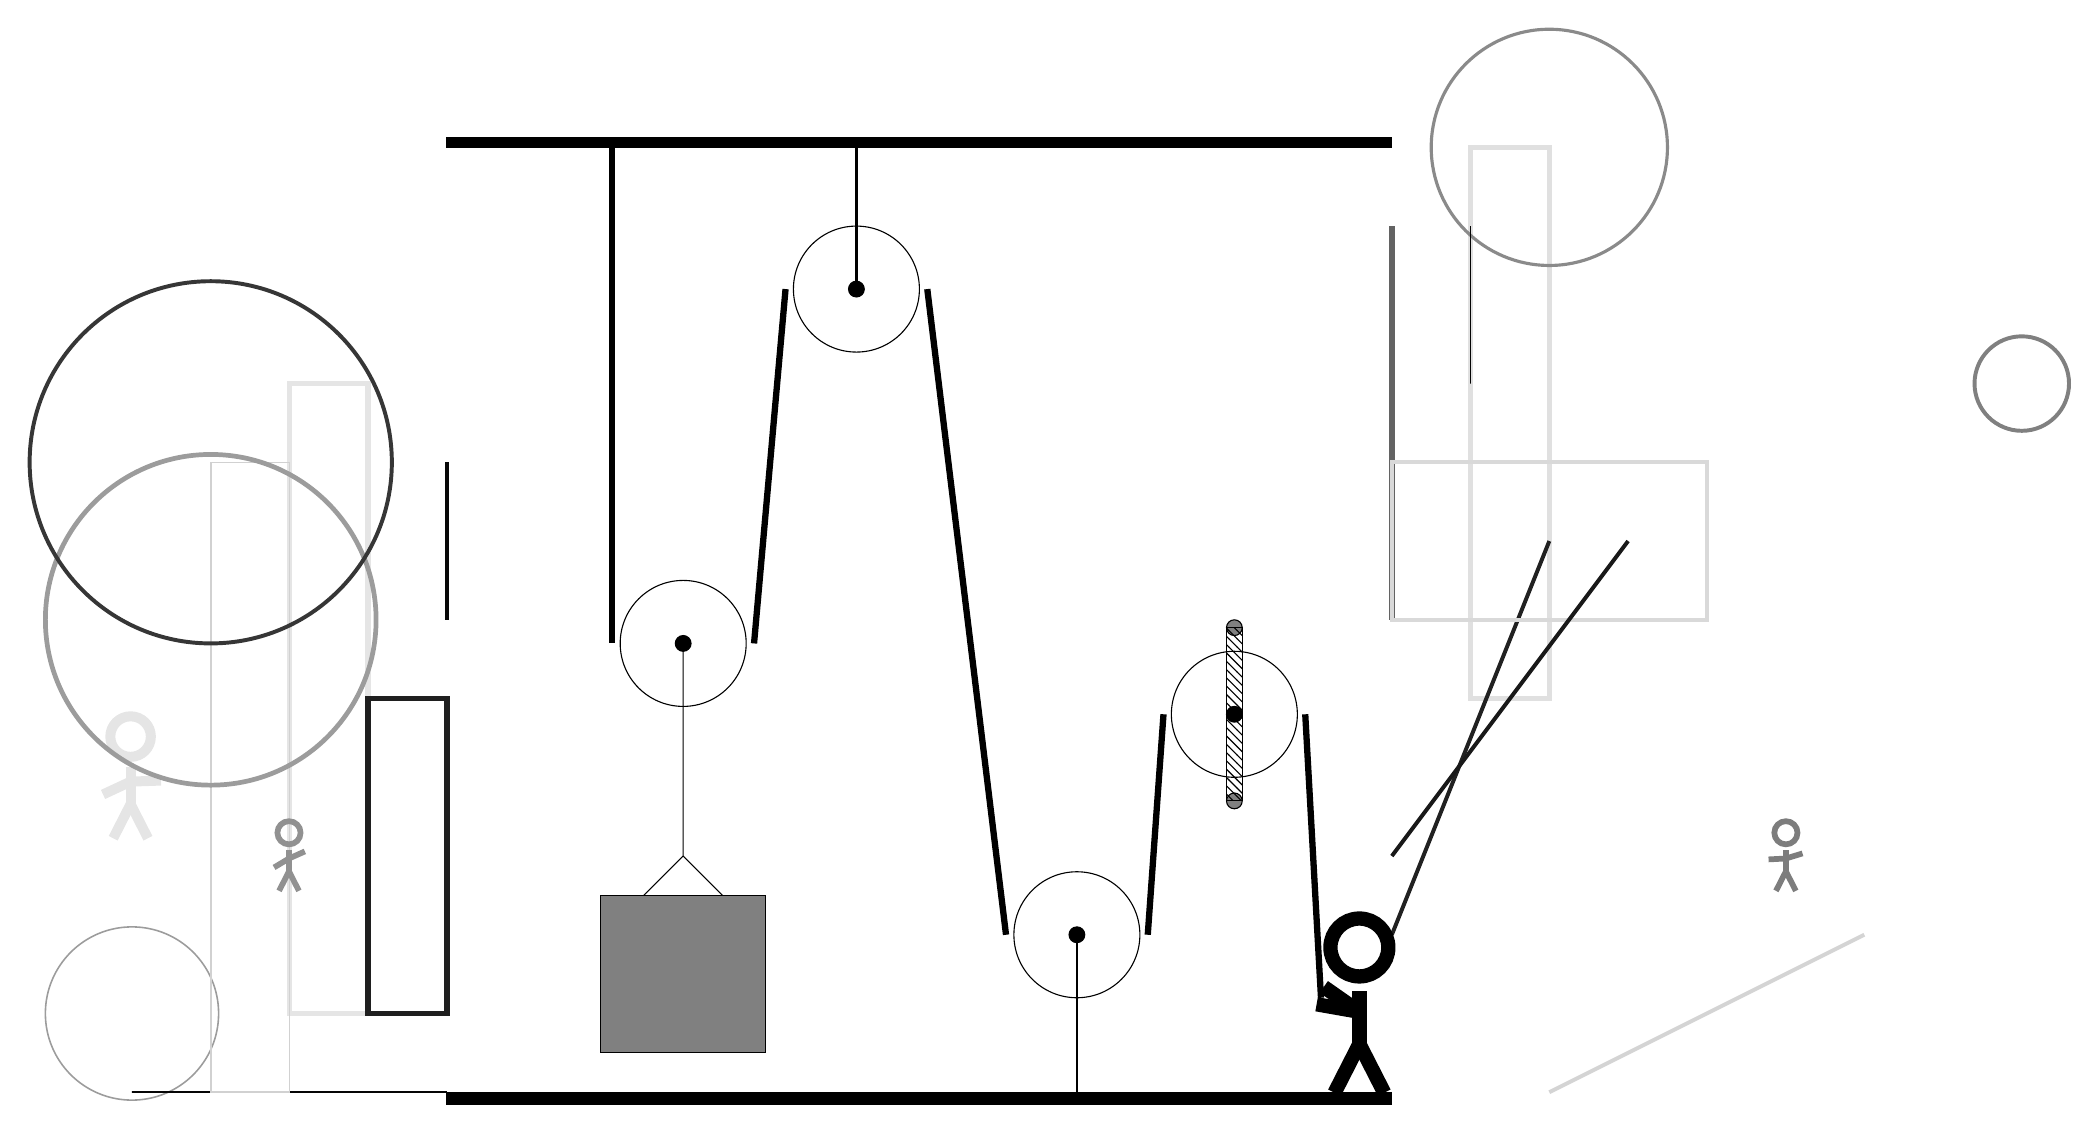
\begin{tikzpicture}
			%%%%% START %%%%%
			
			\draw[fill=black] (-2, 9) rectangle (10, 9.125);
			
			\draw [line width=0.2mm, color=black!39](-6, -2) circle (1.1);
			
			\node[line width=0.2mm, color=black!10] at (-6, 1) {\Strichmaxerl[7][25][2]};
			\draw[line width=0.7mm, color=black!12] (12, 9) rectangle (11, 2);
			\draw[line width=0.3mm, color=black!98] (-2, -3) rectangle (-6, -3);
			\node[line width=0.6mm, color=black!51] at (15, 0) {\Strichmaxerl[4][3][17]};
			
			\draw[line width=0.7mm, color=black!10] (-3, 6) rectangle (-4, -2);
			\draw[line width=0.7mm, color=black!61] (10, 3) rectangle (10, 8);
			\draw [line width=0.4mm, color=black!46](12, 9) circle (1.5);
			\draw[line width=0.5mm, color=black!87](10, -1) -- (12, 4);
			\draw[line width=0.2mm, color=black!18] (-4, -3) rectangle (-5, 5);
			
			\draw[line width=0.2mm, color=black!98] (11, 8) rectangle (11, 6);
			\draw[line width=0.7mm, color=black!88] (-3, 2) rectangle (-2, -2);
			\draw[line width=0.5mm, color=black!15] (10, 5) rectangle (14, 3);
			
			\draw [line width=0.6mm, color=black!39](-5, 3) circle (2.1);
			\draw[line width=0.5mm, color=black!90](10, 0) -- (13, 4);
			\node[line width=0.2mm, color=black!43] at (-4, 0) {\Strichmaxerl[4][31][24]};
			\draw [line width=0.5mm, color=black!50](18, 6) circle (0.6);
			
			\draw[line width=0.5mm, color=black!17](12, -3) -- (16, -1);
			\draw[line width=0.5mm, color=black!97](-2, 5) -- (-2, 3);
			\draw [line width=0.5mm, color=black!79](-5, 5) circle (2.3);
			
			\draw (1, 2.7) circle (0.8);
			\draw[fill=black] (1, 2.7) circle (0.1);
			
			\draw (3.2, 7.2) circle (0.8);
			\draw[fill=black] (3.2, 7.2) circle (0.1);
			\draw[thick] (3.2, 7.2) -- (3.2, 9);
			
			\draw (6, -1) circle (0.8);
			\draw[fill=black] (6, -1) circle (0.1);
			\draw[thick] (6, -1) -- (6, -3);
			
			\draw[fill=white](8, 1.8) circle (0.8);
			\draw[fill=black] (8, 1.8) circle (0.1);
			\draw[fill=black!50] (8, 2.9) circle (0.1);
			\draw[fill=black!50] (8, 0.7) circle (0.1);
			\draw[pattern=north west lines, pattern color=black] (7.9, 2.9) rectangle (8.1, 0.7);
			
			\draw (1, 2.7) -- (1, 0) -- (0.5, -0.5);
			\draw (1, 0) -- (1.5, -0.5);
			\draw[fill=black!50] (-0.05, -0.5) rectangle (2.05, -2.5);
			
			\draw[line width=0.8mm] (0.1, 9) -- (0.1, 2.7);
			\centerarc[line width=0.8mm](1, 2.7)(180:360:0.9);
			\draw[line width=0.8mm](1.9, 2.7) -- (2.3, 7.2);
			\centerarc[line width=0.8mm](3.2, 7.2)(0:180:0.9);
			\draw[line width=0.8mm](4.1, 7.2) -- (5.1, -1);
			\centerarc[line width=0.8mm](6, -1)(180:360:0.9);
			\draw[line width=0.8mm](6.9, -1) -- (7.1, 1.8);
			\centerarc[line width=0.8mm](8, 1.8)(0:180:0.9);
			\draw[line width=0.8mm](8.9, 1.8) -- (9.1, -1.8);
			
			\node at (9.5, -1.9) {\Strichmaxerl[10][-35][170]};
			
			\draw[fill=black] (-2, -3) rectangle (10, -3.15);
			
			%%%%% END %%%%%
		\end{tikzpicture}
	\end{figure}	
\end{document}